\documentclass[border=4pt]{standalone}
% Shared by the independently buildable vector figures.
\usepackage[T1]{fontenc}
\usepackage{amsmath,amssymb,newpxtext,newpxmath}
\usepackage[semibold]{sourcesans}
\usepackage{pgfplots}
\pgfplotsset{compat=1.18}
\usetikzlibrary{arrows.meta,calc,positioning}
\usepgfplotslibrary{groupplots}
\definecolor{ink}{HTML}{19303A}
\definecolor{sea}{HTML}{00675E}
\definecolor{clay}{HTML}{A24725}
\definecolor{muted}{HTML}{4C636C}
\definecolor{rulegray}{HTML}{CAD4D4}
\definecolor{wash}{HTML}{EAF4F0}
\definecolor{warm}{HTML}{F7EEE5}
\color{ink}
\tikzset{every picture/.style={font=\sffamily\small},
  arrow/.style={-{Stealth[length=2mm]},line width=.8pt,draw=muted}}
\pgfplotsset{companion/.style={axis lines=left,axis line style={draw=muted},
  tick style={draw=muted},ticklabel style={font=\sffamily\footnotesize,text=muted},
  label style={font=\sffamily\small},grid=major,grid style={draw=rulegray!64,line width=.25pt},
  tick align=outside,enlarge x limits=false,scaled ticks=false,
  every axis plot/.append style={line join=round},
  legend style={draw=none,fill=none,font=\sffamily\footnotesize},
  title style={font=\sffamily\bfseries\small,anchor=south west,at={(0,1.03)}}}}

\begin{document}
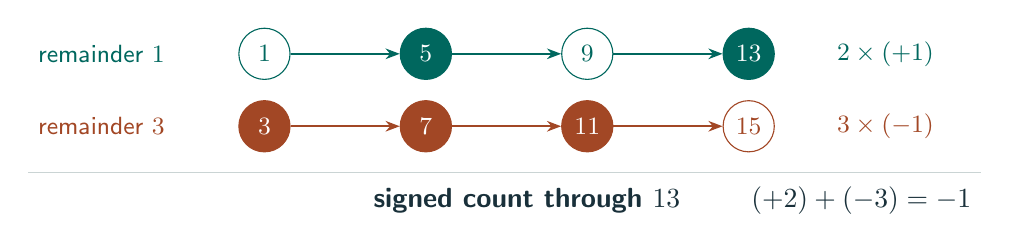
\begin{tikzpicture}[x=1cm,y=1cm,
  number/.style={circle,draw,minimum size=6.5mm,inner sep=1pt},
  counted/.style={draw=\tone,fill=\tone,text=white},
  uncounted/.style={draw=\tone,text=\tone},
  class arrow/.style={-{Stealth[length=1.8mm]},line width=.65pt}]
\foreach \remainder/\y/\tone/\tally/\entries in {
  1/.56/sea/{$2\times(+1)$}/{1/uncounted,5/counted,9/uncounted,13/counted},
  3/-.36/clay/{$3\times(-1)$}/{3/counted,7/counted,11/counted,15/uncounted}}{
  \node[anchor=west,text=\tone] at (0,\y) {remainder $\remainder$};
  \foreach \entry/\markstyle [count=\j from 0] in \entries {
    \node[number,\markstyle] (n\remainder-\j) at ({3+2.05*\j},\y) {$\entry$};
  }
  \foreach \j/\k in {0/1,1/2,2/3}{
    \draw[class arrow,color=\tone] (n\remainder-\j.east) -- (n\remainder-\k.west);
  }
  \node[anchor=west,text=\tone] at (10.15,\y) {\tally};
}
\draw[rulegray] (0,-.95) -- (12.1,-.95);
\node[anchor=east,font=\sffamily\bfseries,text=ink] at (12.1,-1.3)
  {signed count through $13$ \qquad $(+2)+(-3)=-1$};
\end{tikzpicture}
\end{document}
